% -*- root: ../../main.tex -*-
\section{Client Server}
\label{sec:client_server_design}
La realizzazione della modalità di gioco \textbf{multiplayer} richiede di elaborare una struttura che permetta a due o più giocatori di interagire \textbf{contemporaneamente} con la medesima partita. Come introdotto in \ref{subsec:client_server} si è scelto di realizzare un sistema multi-giocatore con le seguenti caratteristiche:
\begin{itemize}
    \item I giocatori interagiscono con il gioco da istanze separate.
    \item La gestione del sistema è centralizzata e la partita è gestita da un Server.
\end{itemize}

Per gestire l'interazione tra il Server e i Client era necessario disporre di un canale di comunicazione tra di essi. Per concretizzare ciò si è scelto di utilizzare un approccio ad attori, introducendo \textit{ClientActor} e \textit{ServerActor}. 

La modellazione dell'architettura Client-Server è stata realizzata come raffigurato in \ref{fig:Controller-Actors-Interaction}:
\begin{figure}[H]
	\centering
	\includegraphics[width=0.99\columnwidth]{drawio/client-server/Controller-Actors-Interaction.pdf}
	\caption{Diagramma delle classi che rappresenta le connessioni tra il Controller e gli attori Client e Server.}
	\label{fig:Controller-Actors-Interaction}
\end{figure}
La struttura del diagramma si presenta con due elementi principali: gli \textbf{attori} e il \textbf{Controller}.
\begin{itemize}
    \item \textbf{Controller:} rappresenta il punto di snodo dello schema ed espone, tra le altre cose, i metodi necessari per gestire le informazioni che arrivano dal \texttt{ClientActor} o dal \texttt{ServerActor}, a seconda della modalità in cui si vuole giocare. Questi metodi sono incapsulati nell'interfaccia \texttt{ActorController}, che viene estesa dal \texttt{ConcreteController}
    \item \textbf{Attori:}
\end{itemize}

\subsection{Sequenza di Join}

Normalmente le interazioni tra client e server si svolgono seguendo una successione di \textbf{step} ben definita:

\begin{enumerate}
    \item Una determinata istanza di gioco diventa Server
    \item Un insieme di istanze di gioco diviene Client
    \item Il server imposta la lobby
    \item Il server crea la lobby e si mette in attesa
    \item Ogni client interessato effettua la richiesta di join alla lobby
    \item Il server risponde con un messaggio di approvazione se la lobby non è ancora piena
    \item Una volta che la lobby è completa il Server attende lo status ready di ogni Client
    \item Una volta che tutti i client sono ready il server comunica a tutti i client la partenza del gioco e distrugge la lobby
    \item Da adesso la partita è in corso per ogni istanza di gioco coinvolta
    \item Ogni client invia i propri comandi al Server
    \item Il Server inserisce la propria azione, calcola il nuovo mondo e lo invia a tutti i client
    \item Una volta che la partita si conclude il server calcola i punteggi e li invia a ogni client e la connessione viene chiusa
\end{enumerate}

Queste interazioni sono anche riportate in forma visiva nello schema: \ref{fig:sequenceClientServer}

\begin{figure}[H]
	\centering
	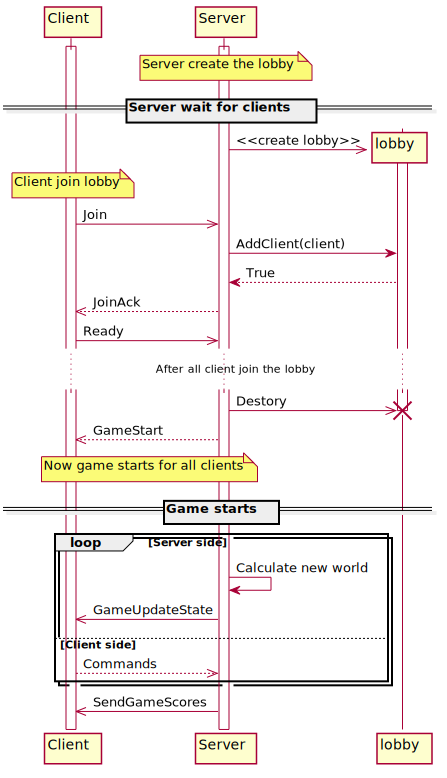
\includegraphics[width=0.99\columnwidth]{plantuml/rendered/sequenceDiagrams/sequenceClientServer.pdf}
	\caption{Diagramma di sequenza che rappresenta la fase di join alla partita e lo svolgimento di essa.}
	\label{fig:sequenceClientServer}
\end{figure}


